\documentclass[twoside]{book}

% Packages required by doxygen
\usepackage{fixltx2e}
\usepackage{calc}
\usepackage{doxygen}
\usepackage[export]{adjustbox} % also loads graphicx
\usepackage{graphicx}
\usepackage[utf8]{inputenc}
\usepackage{makeidx}
\usepackage{multicol}
\usepackage{multirow}
\PassOptionsToPackage{warn}{textcomp}
\usepackage{textcomp}
\usepackage[nointegrals]{wasysym}
\usepackage[table]{xcolor}

% Font selection
\usepackage[T1]{fontenc}
\usepackage[scaled=.90]{helvet}
\usepackage{courier}
\usepackage{amssymb}
\usepackage{sectsty}
\renewcommand{\familydefault}{\sfdefault}
\allsectionsfont{%
  \fontseries{bc}\selectfont%
  \color{darkgray}%
}
\renewcommand{\DoxyLabelFont}{%
  \fontseries{bc}\selectfont%
  \color{darkgray}%
}
\newcommand{\+}{\discretionary{\mbox{\scriptsize$\hookleftarrow$}}{}{}}

% Page & text layout
\usepackage{geometry}
\geometry{%
  a4paper,%
  top=2.5cm,%
  bottom=2.5cm,%
  left=2.5cm,%
  right=2.5cm%
}
\tolerance=750
\hfuzz=15pt
\hbadness=750
\setlength{\emergencystretch}{15pt}
\setlength{\parindent}{0cm}
\setlength{\parskip}{3ex plus 2ex minus 2ex}
\makeatletter
\renewcommand{\paragraph}{%
  \@startsection{paragraph}{4}{0ex}{-1.0ex}{1.0ex}{%
    \normalfont\normalsize\bfseries\SS@parafont%
  }%
}
\renewcommand{\subparagraph}{%
  \@startsection{subparagraph}{5}{0ex}{-1.0ex}{1.0ex}{%
    \normalfont\normalsize\bfseries\SS@subparafont%
  }%
}
\makeatother

% Headers & footers
\usepackage{fancyhdr}
\pagestyle{fancyplain}
\fancyhead[LE]{\fancyplain{}{\bfseries\thepage}}
\fancyhead[CE]{\fancyplain{}{}}
\fancyhead[RE]{\fancyplain{}{\bfseries\leftmark}}
\fancyhead[LO]{\fancyplain{}{\bfseries\rightmark}}
\fancyhead[CO]{\fancyplain{}{}}
\fancyhead[RO]{\fancyplain{}{\bfseries\thepage}}
\fancyfoot[LE]{\fancyplain{}{}}
\fancyfoot[CE]{\fancyplain{}{}}
\fancyfoot[RE]{\fancyplain{}{\bfseries\scriptsize Generated by Doxygen }}
\fancyfoot[LO]{\fancyplain{}{\bfseries\scriptsize Generated by Doxygen }}
\fancyfoot[CO]{\fancyplain{}{}}
\fancyfoot[RO]{\fancyplain{}{}}
\renewcommand{\footrulewidth}{0.4pt}
\renewcommand{\chaptermark}[1]{%
  \markboth{#1}{}%
}
\renewcommand{\sectionmark}[1]{%
  \markright{\thesection\ #1}%
}

% Indices & bibliography
\usepackage{natbib}
\usepackage[titles]{tocloft}
\setcounter{tocdepth}{3}
\setcounter{secnumdepth}{5}
\makeindex

% Hyperlinks (required, but should be loaded last)
\usepackage{ifpdf}
\ifpdf
  \usepackage[pdftex,pagebackref=true]{hyperref}
\else
  \usepackage[ps2pdf,pagebackref=true]{hyperref}
\fi
\hypersetup{%
  colorlinks=true,%
  linkcolor=blue,%
  citecolor=blue,%
  unicode%
}

% Custom commands
\newcommand{\clearemptydoublepage}{%
  \newpage{\pagestyle{empty}\cleardoublepage}%
}

\usepackage{caption}
\captionsetup{labelsep=space,justification=centering,font={bf},singlelinecheck=off,skip=4pt,position=top}

%===== C O N T E N T S =====

\begin{document}

% Titlepage & ToC
\hypersetup{pageanchor=false,
             bookmarksnumbered=true,
             pdfencoding=unicode
            }
\pagenumbering{roman}
\begin{titlepage}
\vspace*{7cm}
\begin{center}%
{\Large cdn-\/webcache }\\
\vspace*{1cm}
{\large Generated by Doxygen 1.8.11}\\
\end{center}
\end{titlepage}
\clearemptydoublepage
\tableofcontents
\clearemptydoublepage
\pagenumbering{arabic}
\hypersetup{pageanchor=true}

%--- Begin generated contents ---
\chapter{cdn-\/webcache}
\label{md__home_ral_workspace_TID_cdn-webcache_README}
\hypertarget{md__home_ral_workspace_TID_cdn-webcache_README}{}
\input{md__home_ral_workspace_TID_cdn-webcache_README}
\chapter{Class Index}
\section{Class List}
Here are the classes, structs, unions and interfaces with brief descriptions\+:\begin{DoxyCompactList}
\item\contentsline{section}{\hyperlink{structngx__http__tcdn__webcache__loc__conf__s}{ngx\+\_\+http\+\_\+tcdn\+\_\+webcache\+\_\+loc\+\_\+conf\+\_\+s} }{\pageref{structngx__http__tcdn__webcache__loc__conf__s}}{}
\item\contentsline{section}{\hyperlink{structsync__tracker__thr__ctx__s}{sync\+\_\+tracker\+\_\+thr\+\_\+ctx\+\_\+s} }{\pageref{structsync__tracker__thr__ctx__s}}{}
\end{DoxyCompactList}

\chapter{File Index}
\section{File List}
Here is a list of all documented files with brief descriptions\+:\begin{DoxyCompactList}
\item\contentsline{section}{\hyperlink{ngx__http__tcdn__webcache__module_8c}{ngx\+\_\+http\+\_\+tcdn\+\_\+webcache\+\_\+module.\+c} \\*T\+C\+D\+N-\/webcache module for Nginx }{\pageref{ngx__http__tcdn__webcache__module_8c}}{}
\end{DoxyCompactList}

\chapter{Class Documentation}
\hypertarget{structngx__http__tcdn__webcache__loc__conf__s}{}\section{ngx\+\_\+http\+\_\+tcdn\+\_\+webcache\+\_\+loc\+\_\+conf\+\_\+s Struct Reference}
\label{structngx__http__tcdn__webcache__loc__conf__s}\index{ngx\+\_\+http\+\_\+tcdn\+\_\+webcache\+\_\+loc\+\_\+conf\+\_\+s@{ngx\+\_\+http\+\_\+tcdn\+\_\+webcache\+\_\+loc\+\_\+conf\+\_\+s}}
\subsection*{Public Attributes}
\begin{DoxyCompactItemize}
\item 
ngx\+\_\+uint\+\_\+t \hyperlink{structngx__http__tcdn__webcache__loc__conf__s_a9730c60ca294166a96154e7ada19a3ec}{bucket\+\_\+json\+\_\+refresh\+\_\+period\+\_\+secs}
\item 
uint64\+\_\+t \hyperlink{structngx__http__tcdn__webcache__loc__conf__s_a3ea999ac7a3d6d325d3101658677706c}{bucket\+\_\+json\+\_\+monot\+\_\+ts\+\_\+secs}
\item 
ngx\+\_\+pool\+\_\+t $\ast$ \hyperlink{structngx__http__tcdn__webcache__loc__conf__s_a94064da09d7e03102f9906f20b139e6e}{pool}
\item 
ngx\+\_\+thread\+\_\+pool\+\_\+t $\ast$ \hyperlink{structngx__http__tcdn__webcache__loc__conf__s_a45fb29b1a518f86433416c1798d6bef9}{ngx\+\_\+thread\+\_\+pool}
\end{DoxyCompactItemize}


\subsection{Detailed Description}
T\+C\+D\+N-\/webcache module\textquotesingle{}s location configuration context structure. The fields in this structure are thought to be initially configured through Nginx\textquotesingle{}s configuration file, and lately by any other dynamic run-\/time mean. Apart from configurations settings, this structure will also hold status or data fields to be used persistently by this module. 

Definition at line 65 of file ngx\+\_\+http\+\_\+tcdn\+\_\+webcache\+\_\+module.\+c.



\subsection{Member Data Documentation}
\index{ngx\+\_\+http\+\_\+tcdn\+\_\+webcache\+\_\+loc\+\_\+conf\+\_\+s@{ngx\+\_\+http\+\_\+tcdn\+\_\+webcache\+\_\+loc\+\_\+conf\+\_\+s}!bucket\+\_\+json\+\_\+monot\+\_\+ts\+\_\+secs@{bucket\+\_\+json\+\_\+monot\+\_\+ts\+\_\+secs}}
\index{bucket\+\_\+json\+\_\+monot\+\_\+ts\+\_\+secs@{bucket\+\_\+json\+\_\+monot\+\_\+ts\+\_\+secs}!ngx\+\_\+http\+\_\+tcdn\+\_\+webcache\+\_\+loc\+\_\+conf\+\_\+s@{ngx\+\_\+http\+\_\+tcdn\+\_\+webcache\+\_\+loc\+\_\+conf\+\_\+s}}
\subsubsection[{\texorpdfstring{bucket\+\_\+json\+\_\+monot\+\_\+ts\+\_\+secs}{bucket_json_monot_ts_secs}}]{\setlength{\rightskip}{0pt plus 5cm}uint64\+\_\+t ngx\+\_\+http\+\_\+tcdn\+\_\+webcache\+\_\+loc\+\_\+conf\+\_\+s\+::bucket\+\_\+json\+\_\+monot\+\_\+ts\+\_\+secs}\hypertarget{structngx__http__tcdn__webcache__loc__conf__s_a3ea999ac7a3d6d325d3101658677706c}{}\label{structngx__http__tcdn__webcache__loc__conf__s_a3ea999ac7a3d6d325d3101658677706c}
Monotonic time-\/stamp, in seconds, indicating the date when \textquotesingle{}bucket.\+json\textquotesingle{} was updated for the last time. If this value is older than a specific refresh period, the bucket should be requested and parsed again. 

Definition at line 76 of file ngx\+\_\+http\+\_\+tcdn\+\_\+webcache\+\_\+module.\+c.

\index{ngx\+\_\+http\+\_\+tcdn\+\_\+webcache\+\_\+loc\+\_\+conf\+\_\+s@{ngx\+\_\+http\+\_\+tcdn\+\_\+webcache\+\_\+loc\+\_\+conf\+\_\+s}!bucket\+\_\+json\+\_\+refresh\+\_\+period\+\_\+secs@{bucket\+\_\+json\+\_\+refresh\+\_\+period\+\_\+secs}}
\index{bucket\+\_\+json\+\_\+refresh\+\_\+period\+\_\+secs@{bucket\+\_\+json\+\_\+refresh\+\_\+period\+\_\+secs}!ngx\+\_\+http\+\_\+tcdn\+\_\+webcache\+\_\+loc\+\_\+conf\+\_\+s@{ngx\+\_\+http\+\_\+tcdn\+\_\+webcache\+\_\+loc\+\_\+conf\+\_\+s}}
\subsubsection[{\texorpdfstring{bucket\+\_\+json\+\_\+refresh\+\_\+period\+\_\+secs}{bucket_json_refresh_period_secs}}]{\setlength{\rightskip}{0pt plus 5cm}ngx\+\_\+uint\+\_\+t ngx\+\_\+http\+\_\+tcdn\+\_\+webcache\+\_\+loc\+\_\+conf\+\_\+s\+::bucket\+\_\+json\+\_\+refresh\+\_\+period\+\_\+secs}\hypertarget{structngx__http__tcdn__webcache__loc__conf__s_a9730c60ca294166a96154e7ada19a3ec}{}\label{structngx__http__tcdn__webcache__loc__conf__s_a9730c60ca294166a96154e7ada19a3ec}
Specifies the refresh period, in seconds, for the \textquotesingle{}bucket.\+json\textquotesingle{}. 

Definition at line 69 of file ngx\+\_\+http\+\_\+tcdn\+\_\+webcache\+\_\+module.\+c.

\index{ngx\+\_\+http\+\_\+tcdn\+\_\+webcache\+\_\+loc\+\_\+conf\+\_\+s@{ngx\+\_\+http\+\_\+tcdn\+\_\+webcache\+\_\+loc\+\_\+conf\+\_\+s}!ngx\+\_\+thread\+\_\+pool@{ngx\+\_\+thread\+\_\+pool}}
\index{ngx\+\_\+thread\+\_\+pool@{ngx\+\_\+thread\+\_\+pool}!ngx\+\_\+http\+\_\+tcdn\+\_\+webcache\+\_\+loc\+\_\+conf\+\_\+s@{ngx\+\_\+http\+\_\+tcdn\+\_\+webcache\+\_\+loc\+\_\+conf\+\_\+s}}
\subsubsection[{\texorpdfstring{ngx\+\_\+thread\+\_\+pool}{ngx_thread_pool}}]{\setlength{\rightskip}{0pt plus 5cm}ngx\+\_\+thread\+\_\+pool\+\_\+t$\ast$ ngx\+\_\+http\+\_\+tcdn\+\_\+webcache\+\_\+loc\+\_\+conf\+\_\+s\+::ngx\+\_\+thread\+\_\+pool}\hypertarget{structngx__http__tcdn__webcache__loc__conf__s_a45fb29b1a518f86433416c1798d6bef9}{}\label{structngx__http__tcdn__webcache__loc__conf__s_a45fb29b1a518f86433416c1798d6bef9}
Pointer to module\textquotesingle{}s thread-\/pool. To enable Nginx\textquotesingle{}s thread pool support, Nginx core {\itshape M\+U\+ST} be compiled with the configuration option \textquotesingle{}--with-\/threads\textquotesingle{}. The pool is used for multi-\/threaded blocking tasks (e.\+g. reading and sending of files) without blocking worker processes. 

Definition at line 91 of file ngx\+\_\+http\+\_\+tcdn\+\_\+webcache\+\_\+module.\+c.

\index{ngx\+\_\+http\+\_\+tcdn\+\_\+webcache\+\_\+loc\+\_\+conf\+\_\+s@{ngx\+\_\+http\+\_\+tcdn\+\_\+webcache\+\_\+loc\+\_\+conf\+\_\+s}!pool@{pool}}
\index{pool@{pool}!ngx\+\_\+http\+\_\+tcdn\+\_\+webcache\+\_\+loc\+\_\+conf\+\_\+s@{ngx\+\_\+http\+\_\+tcdn\+\_\+webcache\+\_\+loc\+\_\+conf\+\_\+s}}
\subsubsection[{\texorpdfstring{pool}{pool}}]{\setlength{\rightskip}{0pt plus 5cm}ngx\+\_\+pool\+\_\+t$\ast$ ngx\+\_\+http\+\_\+tcdn\+\_\+webcache\+\_\+loc\+\_\+conf\+\_\+s\+::pool}\hypertarget{structngx__http__tcdn__webcache__loc__conf__s_a94064da09d7e03102f9906f20b139e6e}{}\label{structngx__http__tcdn__webcache__loc__conf__s_a94064da09d7e03102f9906f20b139e6e}
Pointer to module\textquotesingle{}s dynamic memory pool. 

Definition at line 83 of file ngx\+\_\+http\+\_\+tcdn\+\_\+webcache\+\_\+module.\+c.



The documentation for this struct was generated from the following file\+:\begin{DoxyCompactItemize}
\item 
\hyperlink{ngx__http__tcdn__webcache__module_8c}{ngx\+\_\+http\+\_\+tcdn\+\_\+webcache\+\_\+module.\+c}\end{DoxyCompactItemize}

\hypertarget{structsync__tracker__thr__ctx__s}{}\section{sync\+\_\+tracker\+\_\+thr\+\_\+ctx\+\_\+s Struct Reference}
\label{structsync__tracker__thr__ctx__s}\index{sync\+\_\+tracker\+\_\+thr\+\_\+ctx\+\_\+s@{sync\+\_\+tracker\+\_\+thr\+\_\+ctx\+\_\+s}}
\subsection*{Public Attributes}
\begin{DoxyCompactItemize}
\item 
ngx\+\_\+log\+\_\+t $\ast$ \hyperlink{structsync__tracker__thr__ctx__s_ae978c201761fd1c534646e124e5f3be5}{ngx\+\_\+log}
\end{DoxyCompactItemize}


\subsection{Detailed Description}
Tracker synchronization thread context structure. 

Definition at line 193 of file ngx\+\_\+http\+\_\+tcdn\+\_\+webcache\+\_\+module.\+c.



\subsection{Member Data Documentation}
\index{sync\+\_\+tracker\+\_\+thr\+\_\+ctx\+\_\+s@{sync\+\_\+tracker\+\_\+thr\+\_\+ctx\+\_\+s}!ngx\+\_\+log@{ngx\+\_\+log}}
\index{ngx\+\_\+log@{ngx\+\_\+log}!sync\+\_\+tracker\+\_\+thr\+\_\+ctx\+\_\+s@{sync\+\_\+tracker\+\_\+thr\+\_\+ctx\+\_\+s}}
\subsubsection[{\texorpdfstring{ngx\+\_\+log}{ngx_log}}]{\setlength{\rightskip}{0pt plus 5cm}ngx\+\_\+log\+\_\+t$\ast$ sync\+\_\+tracker\+\_\+thr\+\_\+ctx\+\_\+s\+::ngx\+\_\+log}\hypertarget{structsync__tracker__thr__ctx__s_ae978c201761fd1c534646e124e5f3be5}{}\label{structsync__tracker__thr__ctx__s_ae978c201761fd1c534646e124e5f3be5}
Nxing\textquotesingle{}s log context structure. 

Definition at line 197 of file ngx\+\_\+http\+\_\+tcdn\+\_\+webcache\+\_\+module.\+c.



The documentation for this struct was generated from the following file\+:\begin{DoxyCompactItemize}
\item 
\hyperlink{ngx__http__tcdn__webcache__module_8c}{ngx\+\_\+http\+\_\+tcdn\+\_\+webcache\+\_\+module.\+c}\end{DoxyCompactItemize}

\chapter{File Documentation}
\hypertarget{ngx__http__tcdn__webcache__module_8c}{}\section{ngx\+\_\+http\+\_\+tcdn\+\_\+webcache\+\_\+module.\+c File Reference}
\label{ngx__http__tcdn__webcache__module_8c}\index{ngx\+\_\+http\+\_\+tcdn\+\_\+webcache\+\_\+module.\+c@{ngx\+\_\+http\+\_\+tcdn\+\_\+webcache\+\_\+module.\+c}}


T\+C\+D\+N-\/webcache module for Nginx.  


{\ttfamily \#include $<$ngx\+\_\+config.\+h$>$}\\*
{\ttfamily \#include $<$ngx\+\_\+core.\+h$>$}\\*
{\ttfamily \#include $<$ngx\+\_\+http.\+h$>$}\\*
Include dependency graph for ngx\+\_\+http\+\_\+tcdn\+\_\+webcache\+\_\+module.\+c\+:\nopagebreak
\begin{figure}[H]
\begin{center}
\leavevmode
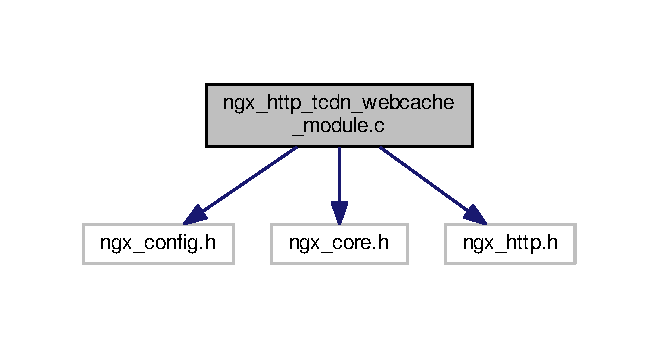
\includegraphics[width=316pt]{ngx__http__tcdn__webcache__module_8c__incl}
\end{center}
\end{figure}
\subsection*{Classes}
\begin{DoxyCompactItemize}
\item 
struct \hyperlink{structngx__http__tcdn__webcache__loc__conf__s}{ngx\+\_\+http\+\_\+tcdn\+\_\+webcache\+\_\+loc\+\_\+conf\+\_\+s}
\item 
struct \hyperlink{structsync__tracker__thr__ctx__s}{sync\+\_\+tracker\+\_\+thr\+\_\+ctx\+\_\+s}
\end{DoxyCompactItemize}
\subsection*{Macros}
\begin{DoxyCompactItemize}
\item 
\#define \hyperlink{ngx__http__tcdn__webcache__module_8c_a4ca78cacaea6e9411d50a8bc3fd83f75}{E\+N\+A\+B\+L\+E\+\_\+\+D\+E\+B\+U\+G\+\_\+\+L\+O\+GS}
\item 
\#define \hyperlink{ngx__http__tcdn__webcache__module_8c_a7a3bff707b06f72f9b956b01259eecb0}{L\+O\+GD}(N\+G\+X\+\_\+\+L\+OG, ...)
\item 
\#define \hyperlink{ngx__http__tcdn__webcache__module_8c_a6c71a346e1280fe78e59e2e909dbf53e}{C\+H\+E\+C\+K\+\_\+\+DO}(C\+O\+ND,  A\+C\+T\+I\+ON)
\end{DoxyCompactItemize}
\subsection*{Typedefs}
\begin{DoxyCompactItemize}
\item 
typedef struct \hyperlink{structngx__http__tcdn__webcache__loc__conf__s}{ngx\+\_\+http\+\_\+tcdn\+\_\+webcache\+\_\+loc\+\_\+conf\+\_\+s} \hyperlink{ngx__http__tcdn__webcache__module_8c_a50235f4fee163761387726e159bf6946}{ngx\+\_\+http\+\_\+tcdn\+\_\+webcache\+\_\+loc\+\_\+conf\+\_\+t}
\item 
typedef struct \hyperlink{structsync__tracker__thr__ctx__s}{sync\+\_\+tracker\+\_\+thr\+\_\+ctx\+\_\+s} \hyperlink{ngx__http__tcdn__webcache__module_8c_a1c354a254db582224ab9aab2992cab51}{sync\+\_\+tracker\+\_\+thr\+\_\+ctx\+\_\+t}
\end{DoxyCompactItemize}
\subsection*{Functions}
\begin{DoxyCompactItemize}
\item 
static void $\ast$ \hyperlink{ngx__http__tcdn__webcache__module_8c_a287d9e7a7069dad9404420a470989ec6}{ngx\+\_\+http\+\_\+tcdn\+\_\+webcache\+\_\+create\+\_\+conf} (ngx\+\_\+conf\+\_\+t $\ast$ngx\+\_\+conf)
\item 
static char $\ast$ \hyperlink{ngx__http__tcdn__webcache__module_8c_a88ddc377ed25c01676820cc1e66432d5}{ngx\+\_\+http\+\_\+tcdn\+\_\+webcache\+\_\+merge\+\_\+conf} (ngx\+\_\+conf\+\_\+t $\ast$ngx\+\_\+conf, void $\ast$parent, void $\ast$child)
\item 
static char $\ast$ \hyperlink{ngx__http__tcdn__webcache__module_8c_aef06b90db04f622a87b3f63fc856a4d6}{ngx\+\_\+http\+\_\+tcdn\+\_\+webcache\+\_\+set\+\_\+handler} (ngx\+\_\+conf\+\_\+t $\ast$ngx\+\_\+conf, ngx\+\_\+command\+\_\+t $\ast$ngx\+\_\+command, void $\ast$opaque\+\_\+loc\+\_\+conf)
\item 
static ngx\+\_\+int\+\_\+t \hyperlink{ngx__http__tcdn__webcache__module_8c_a869f9236672a1ed514370ec2be50207f}{ngx\+\_\+http\+\_\+tcdn\+\_\+webcache\+\_\+handler} (ngx\+\_\+http\+\_\+request\+\_\+t $\ast$r)
\item 
static ngx\+\_\+int\+\_\+t \hyperlink{ngx__http__tcdn__webcache__module_8c_a3d3dbf0946120bd716daae4d2b9741f3}{sync\+\_\+tracker\+\_\+task\+\_\+offload} (\hyperlink{ngx__http__tcdn__webcache__module_8c_a50235f4fee163761387726e159bf6946}{ngx\+\_\+http\+\_\+tcdn\+\_\+webcache\+\_\+loc\+\_\+conf\+\_\+t} $\ast$loc\+\_\+conf, ngx\+\_\+log\+\_\+t $\ast$ngx\+\_\+log)
\item 
static void \hyperlink{ngx__http__tcdn__webcache__module_8c_a04e6d58884c6387c0e5c72a0e720a0a1}{sync\+\_\+tracker\+\_\+thr} (void $\ast$data, ngx\+\_\+log\+\_\+t $\ast$log\+\_\+arg)
\item 
static void \hyperlink{ngx__http__tcdn__webcache__module_8c_aaff59d3b256a188168898f3c90677fee}{sync\+\_\+tracker\+\_\+thr\+\_\+completion} (ngx\+\_\+event\+\_\+t $\ast$ev)
\end{DoxyCompactItemize}
\subsection*{Variables}
\begin{DoxyCompactItemize}
\item 
static ngx\+\_\+command\+\_\+t \hyperlink{ngx__http__tcdn__webcache__module_8c_ad47e068b5af6207ae64febf792480cd5}{ngx\+\_\+http\+\_\+tcdn\+\_\+webcache\+\_\+commands} \mbox{[}$\,$\mbox{]}
\item 
static ngx\+\_\+http\+\_\+module\+\_\+t \hyperlink{ngx__http__tcdn__webcache__module_8c_a2e49aecfdd00d8ce4d031a420167c766}{ngx\+\_\+http\+\_\+tcdn\+\_\+webcache\+\_\+module\+\_\+ctx}
\item 
ngx\+\_\+module\+\_\+t \hyperlink{ngx__http__tcdn__webcache__module_8c_a62111a19c14b897670e142013408c322}{ngx\+\_\+http\+\_\+tcdn\+\_\+webcache\+\_\+module}
\item 
static unsigned char $\ast$ \hyperlink{ngx__http__tcdn__webcache__module_8c_aed3fd45f22376b27c412dbb377192a9f}{thread\+\_\+pool\+\_\+name\+\_\+cstr}
\end{DoxyCompactItemize}


\subsection{Detailed Description}
T\+C\+D\+N-\/webcache module for Nginx. 

\begin{DoxyAuthor}{Author}
Rafael Antoniello 
\end{DoxyAuthor}
\begin{DoxyDate}{Date}
March, 2018 
\end{DoxyDate}


\subsection{Macro Definition Documentation}
\index{ngx\+\_\+http\+\_\+tcdn\+\_\+webcache\+\_\+module.\+c@{ngx\+\_\+http\+\_\+tcdn\+\_\+webcache\+\_\+module.\+c}!C\+H\+E\+C\+K\+\_\+\+DO@{C\+H\+E\+C\+K\+\_\+\+DO}}
\index{C\+H\+E\+C\+K\+\_\+\+DO@{C\+H\+E\+C\+K\+\_\+\+DO}!ngx\+\_\+http\+\_\+tcdn\+\_\+webcache\+\_\+module.\+c@{ngx\+\_\+http\+\_\+tcdn\+\_\+webcache\+\_\+module.\+c}}
\subsubsection[{\texorpdfstring{C\+H\+E\+C\+K\+\_\+\+DO}{CHECK_DO}}]{\setlength{\rightskip}{0pt plus 5cm}\#define C\+H\+E\+C\+K\+\_\+\+DO(
\begin{DoxyParamCaption}
\item[{}]{C\+O\+ND, }
\item[{}]{A\+C\+T\+I\+ON}
\end{DoxyParamCaption}
)}\hypertarget{ngx__http__tcdn__webcache__module_8c_a6c71a346e1280fe78e59e2e909dbf53e}{}\label{ngx__http__tcdn__webcache__module_8c_a6c71a346e1280fe78e59e2e909dbf53e}
{\bfseries Value\+:}
\begin{DoxyCode}
\textcolor{keywordflow}{if}(!(COND)) \{\(\backslash\)
        ngx\_log\_error(NGX\_LOG\_ERR, ngx\_log, 0, \(\backslash\)
            \textcolor{stringliteral}{"%s:%d: Check point failed.\(\backslash\)n"}, \_\_FILE\_\_, \_\_LINE\_\_);\(\backslash\)
        ACTION;\(\backslash\)
    \}
\end{DoxyCode}
Generic trace for tracking check-\/points failures. Thought to be enabled even in release version. 

Definition at line 51 of file ngx\+\_\+http\+\_\+tcdn\+\_\+webcache\+\_\+module.\+c.

\index{ngx\+\_\+http\+\_\+tcdn\+\_\+webcache\+\_\+module.\+c@{ngx\+\_\+http\+\_\+tcdn\+\_\+webcache\+\_\+module.\+c}!E\+N\+A\+B\+L\+E\+\_\+\+D\+E\+B\+U\+G\+\_\+\+L\+O\+GS@{E\+N\+A\+B\+L\+E\+\_\+\+D\+E\+B\+U\+G\+\_\+\+L\+O\+GS}}
\index{E\+N\+A\+B\+L\+E\+\_\+\+D\+E\+B\+U\+G\+\_\+\+L\+O\+GS@{E\+N\+A\+B\+L\+E\+\_\+\+D\+E\+B\+U\+G\+\_\+\+L\+O\+GS}!ngx\+\_\+http\+\_\+tcdn\+\_\+webcache\+\_\+module.\+c@{ngx\+\_\+http\+\_\+tcdn\+\_\+webcache\+\_\+module.\+c}}
\subsubsection[{\texorpdfstring{E\+N\+A\+B\+L\+E\+\_\+\+D\+E\+B\+U\+G\+\_\+\+L\+O\+GS}{ENABLE_DEBUG_LOGS}}]{\setlength{\rightskip}{0pt plus 5cm}\#define E\+N\+A\+B\+L\+E\+\_\+\+D\+E\+B\+U\+G\+\_\+\+L\+O\+GS}\hypertarget{ngx__http__tcdn__webcache__module_8c_a4ca78cacaea6e9411d50a8bc3fd83f75}{}\label{ngx__http__tcdn__webcache__module_8c_a4ca78cacaea6e9411d50a8bc3fd83f75}
Logs for local debugging. Un-\/comment \textquotesingle{}E\+N\+A\+B\+L\+E\+\_\+\+D\+E\+B\+U\+G\+\_\+\+L\+O\+GS\textquotesingle{} to trace. Disable on release version. 

Definition at line 23 of file ngx\+\_\+http\+\_\+tcdn\+\_\+webcache\+\_\+module.\+c.

\index{ngx\+\_\+http\+\_\+tcdn\+\_\+webcache\+\_\+module.\+c@{ngx\+\_\+http\+\_\+tcdn\+\_\+webcache\+\_\+module.\+c}!L\+O\+GD@{L\+O\+GD}}
\index{L\+O\+GD@{L\+O\+GD}!ngx\+\_\+http\+\_\+tcdn\+\_\+webcache\+\_\+module.\+c@{ngx\+\_\+http\+\_\+tcdn\+\_\+webcache\+\_\+module.\+c}}
\subsubsection[{\texorpdfstring{L\+O\+GD}{LOGD}}]{\setlength{\rightskip}{0pt plus 5cm}\#define L\+O\+GD(
\begin{DoxyParamCaption}
\item[{}]{N\+G\+X\+\_\+\+L\+OG, }
\item[{}]{...}
\end{DoxyParamCaption}
)}\hypertarget{ngx__http__tcdn__webcache__module_8c_a7a3bff707b06f72f9b956b01259eecb0}{}\label{ngx__http__tcdn__webcache__module_8c_a7a3bff707b06f72f9b956b01259eecb0}
{\bfseries Value\+:}
\begin{DoxyCode}
\textcolor{keywordflow}{if}((NGX\_LOG)) \{ \(\backslash\)
        ngx\_log\_error(NGX\_LOG\_ERR, NGX\_LOG, 0, \textcolor{stringliteral}{"\(\backslash\)n%s:%d: "}, \(\backslash\)
                \_\_FILE\_\_, \_\_LINE\_\_); \(\backslash\)
        ngx\_log\_error(NGX\_LOG\_ERR, NGX\_LOG, 0, ##\_\_VA\_ARGS\_\_); \(\backslash\)
    \}
\end{DoxyCode}
Log macro for locally debugging. We directly use \textquotesingle{}ngx\+\_\+log\+\_\+error\textquotesingle{} as it is used internally for debugging tracing functions (see for example \textquotesingle{}ngx\+\_\+log\+\_\+debug\textquotesingle{}). Un-\/comment \textquotesingle{}E\+N\+A\+B\+L\+E\+\_\+\+D\+E\+B\+U\+G\+\_\+\+L\+O\+GS\textquotesingle{} to trace. Disable on release version. 

Definition at line 31 of file ngx\+\_\+http\+\_\+tcdn\+\_\+webcache\+\_\+module.\+c.



\subsection{Typedef Documentation}
\index{ngx\+\_\+http\+\_\+tcdn\+\_\+webcache\+\_\+module.\+c@{ngx\+\_\+http\+\_\+tcdn\+\_\+webcache\+\_\+module.\+c}!ngx\+\_\+http\+\_\+tcdn\+\_\+webcache\+\_\+loc\+\_\+conf\+\_\+t@{ngx\+\_\+http\+\_\+tcdn\+\_\+webcache\+\_\+loc\+\_\+conf\+\_\+t}}
\index{ngx\+\_\+http\+\_\+tcdn\+\_\+webcache\+\_\+loc\+\_\+conf\+\_\+t@{ngx\+\_\+http\+\_\+tcdn\+\_\+webcache\+\_\+loc\+\_\+conf\+\_\+t}!ngx\+\_\+http\+\_\+tcdn\+\_\+webcache\+\_\+module.\+c@{ngx\+\_\+http\+\_\+tcdn\+\_\+webcache\+\_\+module.\+c}}
\subsubsection[{\texorpdfstring{ngx\+\_\+http\+\_\+tcdn\+\_\+webcache\+\_\+loc\+\_\+conf\+\_\+t}{ngx_http_tcdn_webcache_loc_conf_t}}]{\setlength{\rightskip}{0pt plus 5cm}typedef struct {\bf ngx\+\_\+http\+\_\+tcdn\+\_\+webcache\+\_\+loc\+\_\+conf\+\_\+s}  {\bf ngx\+\_\+http\+\_\+tcdn\+\_\+webcache\+\_\+loc\+\_\+conf\+\_\+t}}\hypertarget{ngx__http__tcdn__webcache__module_8c_a50235f4fee163761387726e159bf6946}{}\label{ngx__http__tcdn__webcache__module_8c_a50235f4fee163761387726e159bf6946}
T\+C\+D\+N-\/webcache module\textquotesingle{}s location configuration context structure. The fields in this structure are thought to be initially configured through Nginx\textquotesingle{}s configuration file, and lately by any other dynamic run-\/time mean. Apart from configurations settings, this structure will also hold status or data fields to be used persistently by this module. \index{ngx\+\_\+http\+\_\+tcdn\+\_\+webcache\+\_\+module.\+c@{ngx\+\_\+http\+\_\+tcdn\+\_\+webcache\+\_\+module.\+c}!sync\+\_\+tracker\+\_\+thr\+\_\+ctx\+\_\+t@{sync\+\_\+tracker\+\_\+thr\+\_\+ctx\+\_\+t}}
\index{sync\+\_\+tracker\+\_\+thr\+\_\+ctx\+\_\+t@{sync\+\_\+tracker\+\_\+thr\+\_\+ctx\+\_\+t}!ngx\+\_\+http\+\_\+tcdn\+\_\+webcache\+\_\+module.\+c@{ngx\+\_\+http\+\_\+tcdn\+\_\+webcache\+\_\+module.\+c}}
\subsubsection[{\texorpdfstring{sync\+\_\+tracker\+\_\+thr\+\_\+ctx\+\_\+t}{sync_tracker_thr_ctx_t}}]{\setlength{\rightskip}{0pt plus 5cm}typedef struct {\bf sync\+\_\+tracker\+\_\+thr\+\_\+ctx\+\_\+s}  {\bf sync\+\_\+tracker\+\_\+thr\+\_\+ctx\+\_\+t}}\hypertarget{ngx__http__tcdn__webcache__module_8c_a1c354a254db582224ab9aab2992cab51}{}\label{ngx__http__tcdn__webcache__module_8c_a1c354a254db582224ab9aab2992cab51}
Tracker synchronization thread context structure. 

\subsection{Function Documentation}
\index{ngx\+\_\+http\+\_\+tcdn\+\_\+webcache\+\_\+module.\+c@{ngx\+\_\+http\+\_\+tcdn\+\_\+webcache\+\_\+module.\+c}!ngx\+\_\+http\+\_\+tcdn\+\_\+webcache\+\_\+create\+\_\+conf@{ngx\+\_\+http\+\_\+tcdn\+\_\+webcache\+\_\+create\+\_\+conf}}
\index{ngx\+\_\+http\+\_\+tcdn\+\_\+webcache\+\_\+create\+\_\+conf@{ngx\+\_\+http\+\_\+tcdn\+\_\+webcache\+\_\+create\+\_\+conf}!ngx\+\_\+http\+\_\+tcdn\+\_\+webcache\+\_\+module.\+c@{ngx\+\_\+http\+\_\+tcdn\+\_\+webcache\+\_\+module.\+c}}
\subsubsection[{\texorpdfstring{ngx\+\_\+http\+\_\+tcdn\+\_\+webcache\+\_\+create\+\_\+conf(ngx\+\_\+conf\+\_\+t $\ast$ngx\+\_\+conf)}{ngx_http_tcdn_webcache_create_conf(ngx_conf_t *ngx_conf)}}]{\setlength{\rightskip}{0pt plus 5cm}static void $\ast$ ngx\+\_\+http\+\_\+tcdn\+\_\+webcache\+\_\+create\+\_\+conf (
\begin{DoxyParamCaption}
\item[{ngx\+\_\+conf\+\_\+t $\ast$}]{ngx\+\_\+conf}
\end{DoxyParamCaption}
)\hspace{0.3cm}{\ttfamily [static]}}\hypertarget{ngx__http__tcdn__webcache__module_8c_a287d9e7a7069dad9404420a470989ec6}{}\label{ngx__http__tcdn__webcache__module_8c_a287d9e7a7069dad9404420a470989ec6}
Allocates and initializes location configuration context structure. 
\begin{DoxyParams}{Parameters}
{\em ngx\+\_\+conf} & \\
\hline
\end{DoxyParams}


Definition at line 232 of file ngx\+\_\+http\+\_\+tcdn\+\_\+webcache\+\_\+module.\+c.

\index{ngx\+\_\+http\+\_\+tcdn\+\_\+webcache\+\_\+module.\+c@{ngx\+\_\+http\+\_\+tcdn\+\_\+webcache\+\_\+module.\+c}!ngx\+\_\+http\+\_\+tcdn\+\_\+webcache\+\_\+handler@{ngx\+\_\+http\+\_\+tcdn\+\_\+webcache\+\_\+handler}}
\index{ngx\+\_\+http\+\_\+tcdn\+\_\+webcache\+\_\+handler@{ngx\+\_\+http\+\_\+tcdn\+\_\+webcache\+\_\+handler}!ngx\+\_\+http\+\_\+tcdn\+\_\+webcache\+\_\+module.\+c@{ngx\+\_\+http\+\_\+tcdn\+\_\+webcache\+\_\+module.\+c}}
\subsubsection[{\texorpdfstring{ngx\+\_\+http\+\_\+tcdn\+\_\+webcache\+\_\+handler(ngx\+\_\+http\+\_\+request\+\_\+t $\ast$r)}{ngx_http_tcdn_webcache_handler(ngx_http_request_t *r)}}]{\setlength{\rightskip}{0pt plus 5cm}static ngx\+\_\+int\+\_\+t ngx\+\_\+http\+\_\+tcdn\+\_\+webcache\+\_\+handler (
\begin{DoxyParamCaption}
\item[{ngx\+\_\+http\+\_\+request\+\_\+t $\ast$}]{r}
\end{DoxyParamCaption}
)\hspace{0.3cm}{\ttfamily [static]}}\hypertarget{ngx__http__tcdn__webcache__module_8c_a869f9236672a1ed514370ec2be50207f}{}\label{ngx__http__tcdn__webcache__module_8c_a869f9236672a1ed514370ec2be50207f}
Module\textquotesingle{}s request-\/handler function. Nginx\textquotesingle{}s handlers typically do four things\+:
\begin{DoxyEnumerate}
\item get the location configuration,
\item generate an appropriate response,
\item send the response header,
\item and send the body.
\end{DoxyEnumerate}Alternatively, response can be delegated to a proxy server either by using an internal redirection (see \textquotesingle{}ngx\+\_\+http\+\_\+internal\+\_\+redirect()\textquotesingle{}) or by performing a so-\/called sub-\/request (\textquotesingle{}ngx\+\_\+http\+\_\+subrequest\textquotesingle{}). 
\begin{DoxyParams}{Parameters}
{\em r} & H\+T\+TP request context structure (includes information such as request method, U\+RI, and headers). \\
\hline
\end{DoxyParams}


Definition at line 325 of file ngx\+\_\+http\+\_\+tcdn\+\_\+webcache\+\_\+module.\+c.

\index{ngx\+\_\+http\+\_\+tcdn\+\_\+webcache\+\_\+module.\+c@{ngx\+\_\+http\+\_\+tcdn\+\_\+webcache\+\_\+module.\+c}!ngx\+\_\+http\+\_\+tcdn\+\_\+webcache\+\_\+merge\+\_\+conf@{ngx\+\_\+http\+\_\+tcdn\+\_\+webcache\+\_\+merge\+\_\+conf}}
\index{ngx\+\_\+http\+\_\+tcdn\+\_\+webcache\+\_\+merge\+\_\+conf@{ngx\+\_\+http\+\_\+tcdn\+\_\+webcache\+\_\+merge\+\_\+conf}!ngx\+\_\+http\+\_\+tcdn\+\_\+webcache\+\_\+module.\+c@{ngx\+\_\+http\+\_\+tcdn\+\_\+webcache\+\_\+module.\+c}}
\subsubsection[{\texorpdfstring{ngx\+\_\+http\+\_\+tcdn\+\_\+webcache\+\_\+merge\+\_\+conf(ngx\+\_\+conf\+\_\+t $\ast$ngx\+\_\+conf, void $\ast$parent, void $\ast$child)}{ngx_http_tcdn_webcache_merge_conf(ngx_conf_t *ngx_conf, void *parent, void *child)}}]{\setlength{\rightskip}{0pt plus 5cm}static char $\ast$ ngx\+\_\+http\+\_\+tcdn\+\_\+webcache\+\_\+merge\+\_\+conf (
\begin{DoxyParamCaption}
\item[{ngx\+\_\+conf\+\_\+t $\ast$}]{ngx\+\_\+conf, }
\item[{void $\ast$}]{parent, }
\item[{void $\ast$}]{child}
\end{DoxyParamCaption}
)\hspace{0.3cm}{\ttfamily [static]}}\hypertarget{ngx__http__tcdn__webcache__module_8c_a88ddc377ed25c01676820cc1e66432d5}{}\label{ngx__http__tcdn__webcache__module_8c_a88ddc377ed25c01676820cc1e66432d5}
Merge location configuration context structure. 
\begin{DoxyParams}{Parameters}
{\em ngx\+\_\+conf} & \\
\hline
{\em parent} & \\
\hline
{\em child} & \\
\hline
\end{DoxyParams}


Definition at line 267 of file ngx\+\_\+http\+\_\+tcdn\+\_\+webcache\+\_\+module.\+c.

\index{ngx\+\_\+http\+\_\+tcdn\+\_\+webcache\+\_\+module.\+c@{ngx\+\_\+http\+\_\+tcdn\+\_\+webcache\+\_\+module.\+c}!ngx\+\_\+http\+\_\+tcdn\+\_\+webcache\+\_\+set\+\_\+handler@{ngx\+\_\+http\+\_\+tcdn\+\_\+webcache\+\_\+set\+\_\+handler}}
\index{ngx\+\_\+http\+\_\+tcdn\+\_\+webcache\+\_\+set\+\_\+handler@{ngx\+\_\+http\+\_\+tcdn\+\_\+webcache\+\_\+set\+\_\+handler}!ngx\+\_\+http\+\_\+tcdn\+\_\+webcache\+\_\+module.\+c@{ngx\+\_\+http\+\_\+tcdn\+\_\+webcache\+\_\+module.\+c}}
\subsubsection[{\texorpdfstring{ngx\+\_\+http\+\_\+tcdn\+\_\+webcache\+\_\+set\+\_\+handler(ngx\+\_\+conf\+\_\+t $\ast$ngx\+\_\+conf, ngx\+\_\+command\+\_\+t $\ast$ngx\+\_\+command, void $\ast$opaque\+\_\+loc\+\_\+conf)}{ngx_http_tcdn_webcache_set_handler(ngx_conf_t *ngx_conf, ngx_command_t *ngx_command, void *opaque_loc_conf)}}]{\setlength{\rightskip}{0pt plus 5cm}static char $\ast$ ngx\+\_\+http\+\_\+tcdn\+\_\+webcache\+\_\+set\+\_\+handler (
\begin{DoxyParamCaption}
\item[{ngx\+\_\+conf\+\_\+t $\ast$}]{ngx\+\_\+conf, }
\item[{ngx\+\_\+command\+\_\+t $\ast$}]{ngx\+\_\+command, }
\item[{void $\ast$}]{opaque\+\_\+loc\+\_\+conf}
\end{DoxyParamCaption}
)\hspace{0.3cm}{\ttfamily [static]}}\hypertarget{ngx__http__tcdn__webcache__module_8c_aef06b90db04f622a87b3f63fc856a4d6}{}\label{ngx__http__tcdn__webcache__module_8c_aef06b90db04f622a87b3f63fc856a4d6}
Module\textquotesingle{}s request-\/handler setter function. 
\begin{DoxyParams}{Parameters}
{\em ngx\+\_\+conf} & \\
\hline
{\em ngx\+\_\+command} & \\
\hline
{\em opaque\+\_\+loc\+\_\+conf} & \\
\hline
\end{DoxyParams}


Definition at line 289 of file ngx\+\_\+http\+\_\+tcdn\+\_\+webcache\+\_\+module.\+c.

\index{ngx\+\_\+http\+\_\+tcdn\+\_\+webcache\+\_\+module.\+c@{ngx\+\_\+http\+\_\+tcdn\+\_\+webcache\+\_\+module.\+c}!sync\+\_\+tracker\+\_\+task\+\_\+offload@{sync\+\_\+tracker\+\_\+task\+\_\+offload}}
\index{sync\+\_\+tracker\+\_\+task\+\_\+offload@{sync\+\_\+tracker\+\_\+task\+\_\+offload}!ngx\+\_\+http\+\_\+tcdn\+\_\+webcache\+\_\+module.\+c@{ngx\+\_\+http\+\_\+tcdn\+\_\+webcache\+\_\+module.\+c}}
\subsubsection[{\texorpdfstring{sync\+\_\+tracker\+\_\+task\+\_\+offload(ngx\+\_\+http\+\_\+tcdn\+\_\+webcache\+\_\+loc\+\_\+conf\+\_\+t $\ast$loc\+\_\+conf, ngx\+\_\+log\+\_\+t $\ast$ngx\+\_\+log)}{sync_tracker_task_offload(ngx_http_tcdn_webcache_loc_conf_t *loc_conf, ngx_log_t *ngx_log)}}]{\setlength{\rightskip}{0pt plus 5cm}static ngx\+\_\+int\+\_\+t sync\+\_\+tracker\+\_\+task\+\_\+offload (
\begin{DoxyParamCaption}
\item[{{\bf ngx\+\_\+http\+\_\+tcdn\+\_\+webcache\+\_\+loc\+\_\+conf\+\_\+t} $\ast$}]{loc\+\_\+conf, }
\item[{ngx\+\_\+log\+\_\+t $\ast$}]{ngx\+\_\+log}
\end{DoxyParamCaption}
)\hspace{0.3cm}{\ttfamily [static]}}\hypertarget{ngx__http__tcdn__webcache__module_8c_a3d3dbf0946120bd716daae4d2b9741f3}{}\label{ngx__http__tcdn__webcache__module_8c_a3d3dbf0946120bd716daae4d2b9741f3}
Tracker synchronization off-\/load task function. This function allocates and initializes the related resources to finally launch the off-\/load task in a parallel thread of the thread-\/pool defined for this module. 
\begin{DoxyParams}{Parameters}
{\em loc\+\_\+conf} & Module\textquotesingle{}s location configuration structure. \\
\hline
{\em ngx\+\_\+log} & Nginx\textquotesingle{}s log context structure. \\
\hline
\end{DoxyParams}


Definition at line 436 of file ngx\+\_\+http\+\_\+tcdn\+\_\+webcache\+\_\+module.\+c.

\index{ngx\+\_\+http\+\_\+tcdn\+\_\+webcache\+\_\+module.\+c@{ngx\+\_\+http\+\_\+tcdn\+\_\+webcache\+\_\+module.\+c}!sync\+\_\+tracker\+\_\+thr@{sync\+\_\+tracker\+\_\+thr}}
\index{sync\+\_\+tracker\+\_\+thr@{sync\+\_\+tracker\+\_\+thr}!ngx\+\_\+http\+\_\+tcdn\+\_\+webcache\+\_\+module.\+c@{ngx\+\_\+http\+\_\+tcdn\+\_\+webcache\+\_\+module.\+c}}
\subsubsection[{\texorpdfstring{sync\+\_\+tracker\+\_\+thr(void $\ast$data, ngx\+\_\+log\+\_\+t $\ast$log\+\_\+arg)}{sync_tracker_thr(void *data, ngx_log_t *log_arg)}}]{\setlength{\rightskip}{0pt plus 5cm}static void sync\+\_\+tracker\+\_\+thr (
\begin{DoxyParamCaption}
\item[{void $\ast$}]{data, }
\item[{ngx\+\_\+log\+\_\+t $\ast$}]{log\+\_\+arg}
\end{DoxyParamCaption}
)\hspace{0.3cm}{\ttfamily [static]}}\hypertarget{ngx__http__tcdn__webcache__module_8c_a04e6d58884c6387c0e5c72a0e720a0a1}{}\label{ngx__http__tcdn__webcache__module_8c_a04e6d58884c6387c0e5c72a0e720a0a1}
Tracker synchronization thread function. This function is executed in a separate thread of the available thread-\/pool. 
\begin{DoxyParams}{Parameters}
{\em data} & Opaque pointer to our private thread context structure; that is, \textquotesingle{}sync\+\_\+tracker\+\_\+thr\+\_\+ctx\+\_\+t\textquotesingle{}. \\
\hline
{\em log\+\_\+arg} & Nginx\textquotesingle{}s log context structure. \\
\hline
\end{DoxyParams}


Definition at line 387 of file ngx\+\_\+http\+\_\+tcdn\+\_\+webcache\+\_\+module.\+c.

\index{ngx\+\_\+http\+\_\+tcdn\+\_\+webcache\+\_\+module.\+c@{ngx\+\_\+http\+\_\+tcdn\+\_\+webcache\+\_\+module.\+c}!sync\+\_\+tracker\+\_\+thr\+\_\+completion@{sync\+\_\+tracker\+\_\+thr\+\_\+completion}}
\index{sync\+\_\+tracker\+\_\+thr\+\_\+completion@{sync\+\_\+tracker\+\_\+thr\+\_\+completion}!ngx\+\_\+http\+\_\+tcdn\+\_\+webcache\+\_\+module.\+c@{ngx\+\_\+http\+\_\+tcdn\+\_\+webcache\+\_\+module.\+c}}
\subsubsection[{\texorpdfstring{sync\+\_\+tracker\+\_\+thr\+\_\+completion(ngx\+\_\+event\+\_\+t $\ast$ev)}{sync_tracker_thr_completion(ngx_event_t *ev)}}]{\setlength{\rightskip}{0pt plus 5cm}static void sync\+\_\+tracker\+\_\+thr\+\_\+completion (
\begin{DoxyParamCaption}
\item[{ngx\+\_\+event\+\_\+t $\ast$}]{ev}
\end{DoxyParamCaption}
)\hspace{0.3cm}{\ttfamily [static]}}\hypertarget{ngx__http__tcdn__webcache__module_8c_aaff59d3b256a188168898f3c90677fee}{}\label{ngx__http__tcdn__webcache__module_8c_aaff59d3b256a188168898f3c90677fee}
Tracker synchronization thread completion function. This callback is called just after associated off-\/load thread has finished. Important note\+: it is to remark that this function {\itshape IS} executed {\itshape W\+I\+T\+H\+IN} Nginx event loop (not in parallel), so it must be no blocking. 
\begin{DoxyParams}{Parameters}
{\em ev} & \\
\hline
\end{DoxyParams}


Definition at line 412 of file ngx\+\_\+http\+\_\+tcdn\+\_\+webcache\+\_\+module.\+c.



\subsection{Variable Documentation}
\index{ngx\+\_\+http\+\_\+tcdn\+\_\+webcache\+\_\+module.\+c@{ngx\+\_\+http\+\_\+tcdn\+\_\+webcache\+\_\+module.\+c}!ngx\+\_\+http\+\_\+tcdn\+\_\+webcache\+\_\+commands@{ngx\+\_\+http\+\_\+tcdn\+\_\+webcache\+\_\+commands}}
\index{ngx\+\_\+http\+\_\+tcdn\+\_\+webcache\+\_\+commands@{ngx\+\_\+http\+\_\+tcdn\+\_\+webcache\+\_\+commands}!ngx\+\_\+http\+\_\+tcdn\+\_\+webcache\+\_\+module.\+c@{ngx\+\_\+http\+\_\+tcdn\+\_\+webcache\+\_\+module.\+c}}
\subsubsection[{\texorpdfstring{ngx\+\_\+http\+\_\+tcdn\+\_\+webcache\+\_\+commands}{ngx_http_tcdn_webcache_commands}}]{\setlength{\rightskip}{0pt plus 5cm}ngx\+\_\+command\+\_\+t ngx\+\_\+http\+\_\+tcdn\+\_\+webcache\+\_\+commands\mbox{[}$\,$\mbox{]}\hspace{0.3cm}{\ttfamily [static]}}\hypertarget{ngx__http__tcdn__webcache__module_8c_ad47e068b5af6207ae64febf792480cd5}{}\label{ngx__http__tcdn__webcache__module_8c_ad47e068b5af6207ae64febf792480cd5}
{\bfseries Initial value\+:}
\begin{DoxyCode}
= \{
        \{
                ngx\_string(\textcolor{stringliteral}{"tcdn\_webcache"}),
                NGX\_HTTP\_LOC\_CONF|NGX\_CONF\_NOARGS,
                \hyperlink{ngx__http__tcdn__webcache__module_8c_aef06b90db04f622a87b3f63fc856a4d6}{ngx\_http\_tcdn\_webcache\_set\_handler},
                NGX\_HTTP\_LOC\_CONF\_OFFSET,
                0,
                NULL
        \},
        ngx\_null\_command
\}
\end{DoxyCode}
T\+C\+D\+N-\/webcache module\textquotesingle{}s directives\+:~\newline
 Define a set of \char`\"{}commands\char`\"{} this module will be able to handle. Each command is represented by the structure type \textquotesingle{}ngx\+\_\+command\+\_\+t\textquotesingle{} in which it is specified\+: 
\begin{DoxyItemize}
\item The directive\textquotesingle{}s name (string with no spaces)\+:~\newline
 it will be referenced in Nginx\textquotesingle{}s configuration file, for example, as follows\+: 
\begin{DoxyCode}
1 location / \{
2     my\_directive\_name my\_directive\_arg;
3     ...
4 \}
\end{DoxyCode}
  
\item The directive type (string with no spaces)\+:~\newline
 The type refers to a set of flags that indicate where the directive is legal (e.\+g. N\+G\+X\+\_\+\+H\+T\+T\+P\+\_\+(M\+A\+I\+N/\+S\+R\+V/\+L\+O\+C/...)\+\_\+\+C\+O\+NF to indicate the directive is valid in the main/server/location/... configuration respectively) and how many arguments the directive takes (e.\+g. N\+G\+X\+\_\+\+C\+O\+N\+F\+\_\+(N\+O\+A\+R\+G\+S/\+T\+A\+K\+E1/\+T\+A\+K\+E7/...). ~\newline
 Please refer to \textquotesingle{}core/ngx\+\_\+conf\+\_\+file.\+h\textquotesingle{} (\href{https://github.com/nginx/nginx/blob/master/src/core/ngx_conf_file.h}{\tt https\+://github.\+com/nginx/nginx/blob/master/src/core/ngx\+\_\+conf\+\_\+file.\+h}).  
\item The \textquotesingle{}set\textquotesingle{} callback\+:~\newline
 Pointer to a function for setting up part of the module’s configuration; typically this function will translate the arguments passed to this directive and save an appropriate value in its configuration structure. This setup function will be called when the directive is encountered.  
\item Configuration structure identifier\+:~\newline
 This identifier is used to indicate to the \textquotesingle{}set\textquotesingle{} callback in which configuration structure to save/store the data; namely, it tells Nginx whether a value will get saved to the module’s main configuration, server configuration, or location configuration (with N\+G\+X\+\_\+\+H\+T\+T\+P\+\_\+\+M\+A\+I\+N\+\_\+\+C\+O\+N\+F\+\_\+\+O\+F\+F\+S\+ET, N\+G\+X\+\_\+\+H\+T\+T\+P\+\_\+\+S\+R\+V\+\_\+\+C\+O\+N\+F\+\_\+\+O\+F\+F\+S\+ET or N\+G\+X\+\_\+\+H\+T\+T\+P\+\_\+\+L\+O\+C\+\_\+\+C\+O\+N\+F\+\_\+\+O\+F\+F\+S\+ET respectively).  
\item Configuration structure offset\+:~\newline
 Specifies which field of the identified configuration structure to write to. 


\end{DoxyItemize}

Definition at line 138 of file ngx\+\_\+http\+\_\+tcdn\+\_\+webcache\+\_\+module.\+c.

\index{ngx\+\_\+http\+\_\+tcdn\+\_\+webcache\+\_\+module.\+c@{ngx\+\_\+http\+\_\+tcdn\+\_\+webcache\+\_\+module.\+c}!ngx\+\_\+http\+\_\+tcdn\+\_\+webcache\+\_\+module@{ngx\+\_\+http\+\_\+tcdn\+\_\+webcache\+\_\+module}}
\index{ngx\+\_\+http\+\_\+tcdn\+\_\+webcache\+\_\+module@{ngx\+\_\+http\+\_\+tcdn\+\_\+webcache\+\_\+module}!ngx\+\_\+http\+\_\+tcdn\+\_\+webcache\+\_\+module.\+c@{ngx\+\_\+http\+\_\+tcdn\+\_\+webcache\+\_\+module.\+c}}
\subsubsection[{\texorpdfstring{ngx\+\_\+http\+\_\+tcdn\+\_\+webcache\+\_\+module}{ngx_http_tcdn_webcache_module}}]{\setlength{\rightskip}{0pt plus 5cm}ngx\+\_\+module\+\_\+t ngx\+\_\+http\+\_\+tcdn\+\_\+webcache\+\_\+module}\hypertarget{ngx__http__tcdn__webcache__module_8c_a62111a19c14b897670e142013408c322}{}\label{ngx__http__tcdn__webcache__module_8c_a62111a19c14b897670e142013408c322}
{\bfseries Initial value\+:}
\begin{DoxyCode}
= \{
        NGX\_MODULE\_V1,
        &\hyperlink{ngx__http__tcdn__webcache__module_8c_a2e49aecfdd00d8ce4d031a420167c766}{ngx\_http\_tcdn\_webcache\_module\_ctx}, 
        \hyperlink{ngx__http__tcdn__webcache__module_8c_ad47e068b5af6207ae64febf792480cd5}{ngx\_http\_tcdn\_webcache\_commands},     
        NGX\_HTTP\_MODULE,                    
        NULL,                               
        NULL,                               
        NULL,                               
        NULL,                               
        NULL,                               
        NULL,                               
        NULL,                               
        NGX\_MODULE\_V1\_PADDING
\}
\end{DoxyCode}
T\+C\+D\+N-\/webcache module context structure. The nomenclature is always~\newline
 \textquotesingle{}ngx\+\_\+http\+\_\+$<$module name$>$\+\_\+module\textquotesingle{}.~\newline
 This is where all references to the contexts and directives go, as well as other callbacks (exit thread, exit process, etc.). 

Definition at line 175 of file ngx\+\_\+http\+\_\+tcdn\+\_\+webcache\+\_\+module.\+c.

\index{ngx\+\_\+http\+\_\+tcdn\+\_\+webcache\+\_\+module.\+c@{ngx\+\_\+http\+\_\+tcdn\+\_\+webcache\+\_\+module.\+c}!ngx\+\_\+http\+\_\+tcdn\+\_\+webcache\+\_\+module\+\_\+ctx@{ngx\+\_\+http\+\_\+tcdn\+\_\+webcache\+\_\+module\+\_\+ctx}}
\index{ngx\+\_\+http\+\_\+tcdn\+\_\+webcache\+\_\+module\+\_\+ctx@{ngx\+\_\+http\+\_\+tcdn\+\_\+webcache\+\_\+module\+\_\+ctx}!ngx\+\_\+http\+\_\+tcdn\+\_\+webcache\+\_\+module.\+c@{ngx\+\_\+http\+\_\+tcdn\+\_\+webcache\+\_\+module.\+c}}
\subsubsection[{\texorpdfstring{ngx\+\_\+http\+\_\+tcdn\+\_\+webcache\+\_\+module\+\_\+ctx}{ngx_http_tcdn_webcache_module_ctx}}]{\setlength{\rightskip}{0pt plus 5cm}ngx\+\_\+http\+\_\+module\+\_\+t ngx\+\_\+http\+\_\+tcdn\+\_\+webcache\+\_\+module\+\_\+ctx\hspace{0.3cm}{\ttfamily [static]}}\hypertarget{ngx__http__tcdn__webcache__module_8c_a2e49aecfdd00d8ce4d031a420167c766}{}\label{ngx__http__tcdn__webcache__module_8c_a2e49aecfdd00d8ce4d031a420167c766}
{\bfseries Initial value\+:}
\begin{DoxyCode}
= \{
        NULL, 
        NULL, 
        NULL, 
        NULL, 
        NULL, 
        NULL, 
        \hyperlink{ngx__http__tcdn__webcache__module_8c_a287d9e7a7069dad9404420a470989ec6}{ngx\_http\_tcdn\_webcache\_create\_conf}, 
        \hyperlink{ngx__http__tcdn__webcache__module_8c_a88ddc377ed25c01676820cc1e66432d5}{ngx\_http\_tcdn\_webcache\_merge\_conf} 
\}
\end{DoxyCode}
T\+C\+D\+N-\/webcache module\textquotesingle{}s configuration functions context structure. It defines the set of callback functions for creating the three configurations (main, server and location) and merging them together. (refer to \textquotesingle{}ngx\+\_\+http\+\_\+config.\+h\textquotesingle{}; \href{https://github.com/nginx/nginx/blob/master/src/http/ngx_http_config.h}{\tt https\+://github.\+com/nginx/nginx/blob/master/src/http/ngx\+\_\+http\+\_\+config.\+h}) 

Definition at line 157 of file ngx\+\_\+http\+\_\+tcdn\+\_\+webcache\+\_\+module.\+c.

\index{ngx\+\_\+http\+\_\+tcdn\+\_\+webcache\+\_\+module.\+c@{ngx\+\_\+http\+\_\+tcdn\+\_\+webcache\+\_\+module.\+c}!thread\+\_\+pool\+\_\+name\+\_\+cstr@{thread\+\_\+pool\+\_\+name\+\_\+cstr}}
\index{thread\+\_\+pool\+\_\+name\+\_\+cstr@{thread\+\_\+pool\+\_\+name\+\_\+cstr}!ngx\+\_\+http\+\_\+tcdn\+\_\+webcache\+\_\+module.\+c@{ngx\+\_\+http\+\_\+tcdn\+\_\+webcache\+\_\+module.\+c}}
\subsubsection[{\texorpdfstring{thread\+\_\+pool\+\_\+name\+\_\+cstr}{thread_pool_name_cstr}}]{\setlength{\rightskip}{0pt plus 5cm}unsigned char$\ast$ thread\+\_\+pool\+\_\+name\+\_\+cstr\hspace{0.3cm}{\ttfamily [static]}}\hypertarget{ngx__http__tcdn__webcache__module_8c_aed3fd45f22376b27c412dbb377192a9f}{}\label{ngx__http__tcdn__webcache__module_8c_aed3fd45f22376b27c412dbb377192a9f}
{\bfseries Initial value\+:}
\begin{DoxyCode}
= (\textcolor{keywordtype}{unsigned} \textcolor{keywordtype}{char}*)
        \textcolor{stringliteral}{"tcdn\_webcache\_thread\_pool"}
\end{DoxyCode}
Thread-\/pool unambiguous identification name. This name is used in the Nginx\textquotesingle{}s configuration file to set the thread-\/pool characteristics. The configuration syntax is the following (set in the main context)\+:~\newline
 thread\+\_\+pool name threads=number \mbox{[}max\+\_\+queue=number\mbox{]};~\newline
 For example\+: 
\begin{DoxyCode}
1 thread\_pool tcdn\_webcache\_thread\_pool threads=32 max\_queue=65536;
\end{DoxyCode}
 

Definition at line 225 of file ngx\+\_\+http\+\_\+tcdn\+\_\+webcache\+\_\+module.\+c.


%--- End generated contents ---

% Index
\backmatter
\newpage
\phantomsection
\clearemptydoublepage
\addcontentsline{toc}{chapter}{Index}
\printindex

\end{document}
